\documentclass[12pt, a4paper]{extarticle}

\usepackage{geometry}
\usepackage{fancyhdr}
\usepackage{url}
\usepackage{hyperref}
\usepackage{graphicx}
\usepackage{fontspec}
\setmainfont{Comic Sans MS}

\graphicspath{ {images/} }

\pagestyle{fancy}
\fancyhf{}
\rhead{...}
\lhead{sprintplanningen}
\rfoot{\thepage}
\lfoot{}

\title{sprintplanningen}
\date{6-4-2017}
\author{Wicky Bhaggoe}

\begin{document}
	\nocite{*}
	\pagenumbering{gobble}
	\maketitle
	project 7/8
	
	0882135
	
	\newpage
	\tableofcontents
	
	\newpage
	\pagenumbering{arabic}
	\section{sprintplanningen}
	\subsection{sprintplanning 1}
	\begin{center}
		\begin{tabular}{ |c|c|c|c|c|c|c|c|c|c|c| } 
			\hline
			project & story & task & start & day 7 & day 6 & day 5 & day 4& day 3 & day 2 & day 1 \\ 
			my project & story 7 & task 7.2 & 8 & 7 & 7 & 6 & 3 & 0 & 0 & 0 \\
			my project & story 8 & task 8.1 & 13  & 10 & 10 & 6 & 3 & 3 & 0 & 0 \\
			my project & story 11 & task 11.1 & 5 & 2 & 2 & 2 & 0 & 0 & 0 & 0 \\
			my project & story 9 & task 9.1 & 13 & 12 & 10 & 8 & 6 & 3 & 1 & 0 \\
			\hline
		\end{tabular}
	\end{center}

	\begin{center}
	\begin{tabular}{ |c|c|c|c|c|c|c|c| } 
		\hline
		start & day 7 & day 6 & day 5 & day 4& day 3 & day 2 & day 1 \\ 
		38 & 32 & 27 & 21 & 16 & 10 & 5 & 0 \\
		38 & 38 & 36 & 30 & 21 & 15 & 12 & 0 \\
	    \hline
	\end{tabular}
	\end{center}
	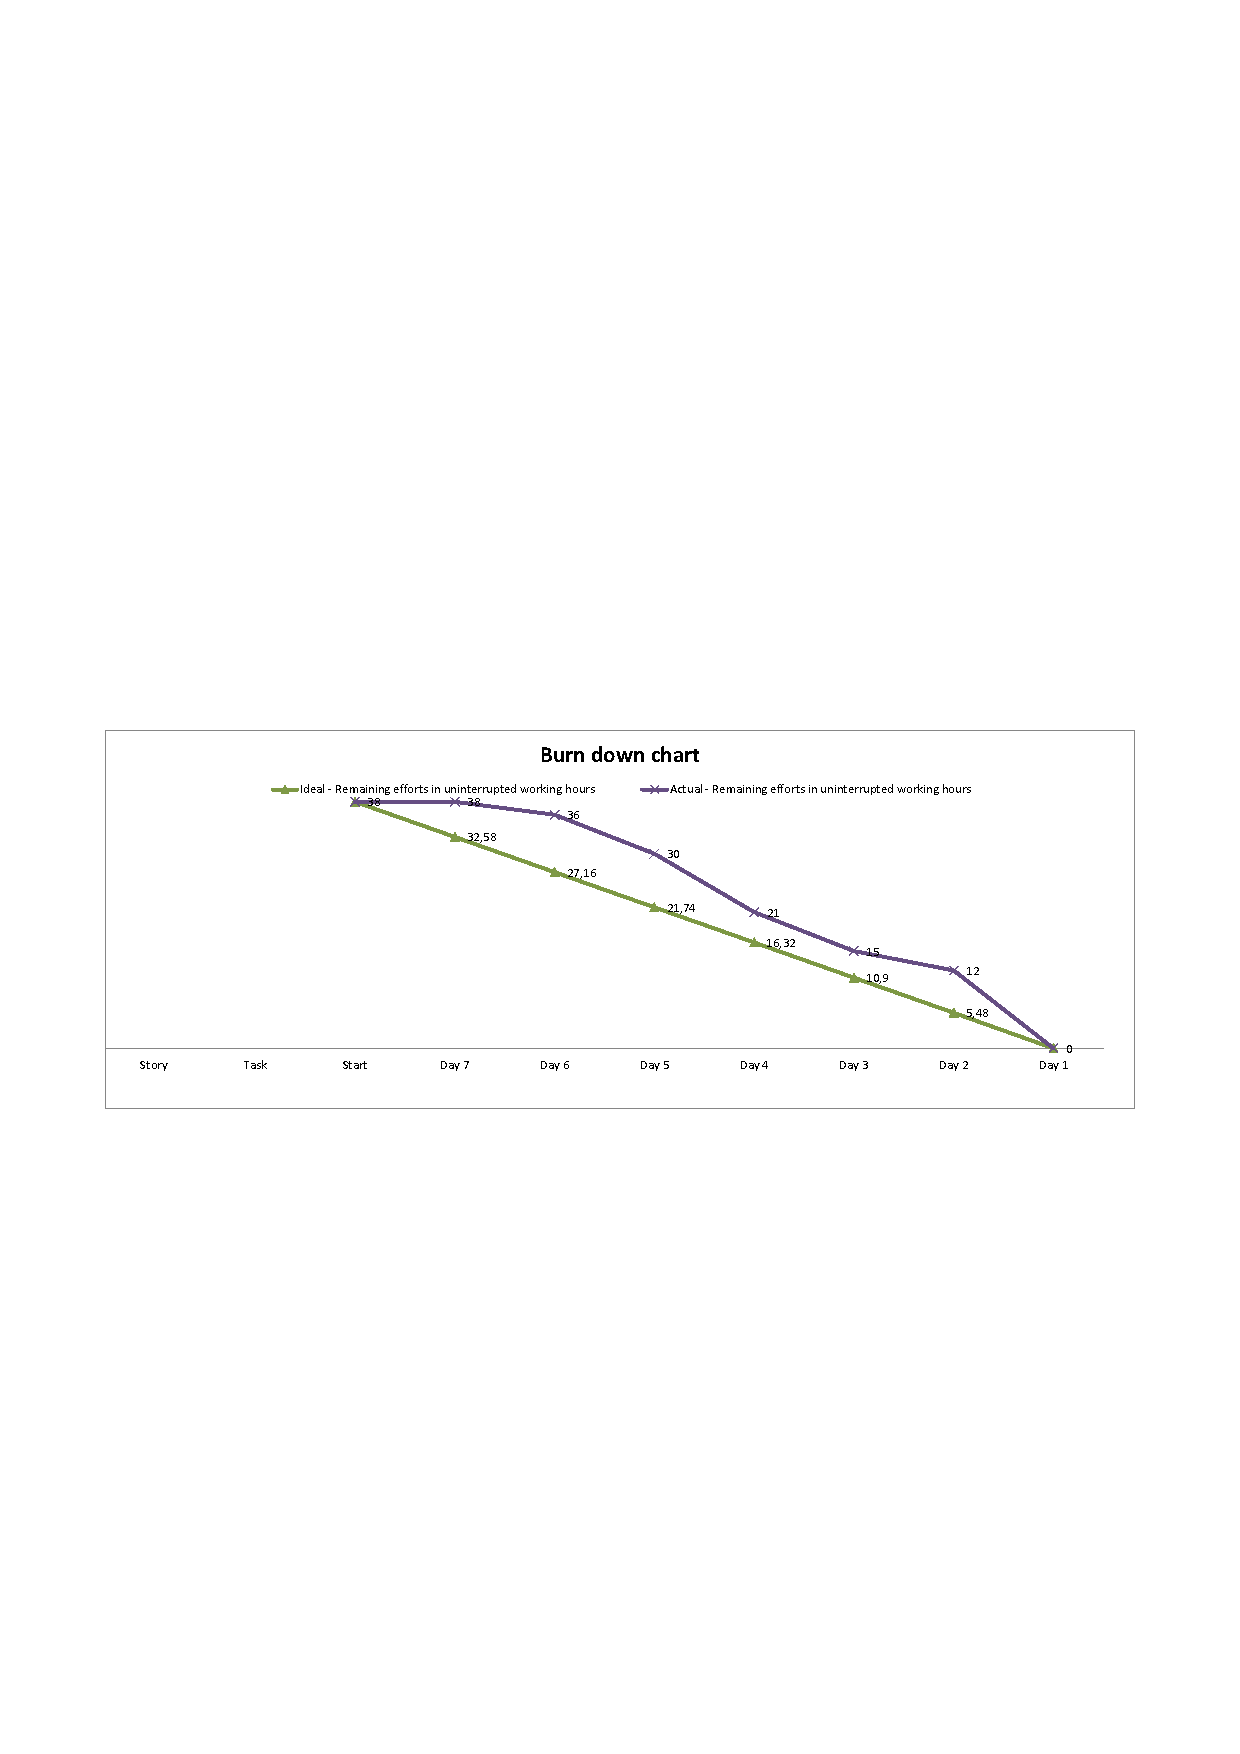
\includegraphics[scale=0.4]{burndownchart}
	\newpage
	\subsection{sprintplanning 2}

  
    
	
	\newpage
	\section{Retrospectives}
	\subsection{Retrospective week 1}
Geef als groep antwoord op de volgende vragen: 
 \newline
Wat was de velocity van de afgelopen sprint?  
 \newline
Wat ging deze sprint goed? 
 \newline 
Wat kan de volgende sprint beter?  
 \vspace{5mm}
 \newline
Wat was de velocity van de sprint? 
 \newline
Collin: precies goed 
 \newline
Matthijs: het was genoeg 
 \newline 
Wicky: het was precies goed   
 \vspace{5mm}
 \newline
Wat ging deze sprint goed?  
 \newline 
Collin: deze week hebben we wat extra tijd ingepland voor de bespreking met de P.O zodat we beter konden voorbereiden  
 \newline 
Matthijs: de taken van het veiligheidsrapport waren goed verdeeld 
 \newline  
Wicky: er is niets slecht gegaan 
 \vspace{5mm}
 \newline
Wat kan de volgende sprint beter? 
 \newline 
Collin: niets 
 \newline 
Matthijs: niets 
 \newline 
Wicky: niets  
 \newline 
	
	
\subsection{Retrospective week 2}
Geef als groep antwoord op de volgende vragen: 
\newline
Wat was de velocity van de afgelopen sprint?  
\newline
Wat ging deze sprint goed? 
\newline 
Wat kan de volgende sprint beter?  
\vspace{5mm}
\newline
Wat was de velocity van de sprint? 
\newline
Collin: 
\newline
Matthijs: 
\newline 
Wicky:   
\vspace{5mm}
\newline
Wat ging deze sprint goed?  
\newline 
Collin: 
\newline 
Matthijs: 
\newline  
Wicky:  
\vspace{5mm}
\newline
Wat kan de volgende sprint beter? 
\newline 
Collin: 
\newline 
Matthijs: 
\newline 
Wicky:  
\newline 
	
	\newpage
	
	\bibliography{rapport}
	\bibliographystyle{ieeetr}
	


\end{document}